%\emph{Image segmentation} is the process of [labelling|colloring|classifying] each pixel in [an|the] image [as belonging to |with the label from] an object present depending on conforming corresponding (Fig~\ref{fig:imageSegmentation}).
\emph{Image segmentation} is the task of labelling each pixel in an image according to the object to which it belongs (Fig~\ref{fig:imageSegmentation}).
We can segment an image by training a classifier on small patches, sliding it across bigger images to obtain per-pixel predictions and assigning each pixel to its highest predicted class.
%~\footnote{For classification, we average score vectors across pixels to obtain a single vector for the bigger image.}
\begin{figure}[h]
	\centering
	\begin{subfigure}{0.26\textwidth}
                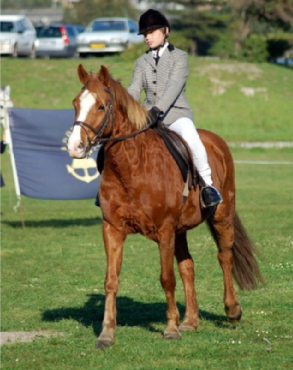
\includegraphics[width=\textwidth]{plots/segmentationImage.png}
		\caption{Original image}
        \end{subfigure}
	~
	\begin{subfigure}{0.26\textwidth}
                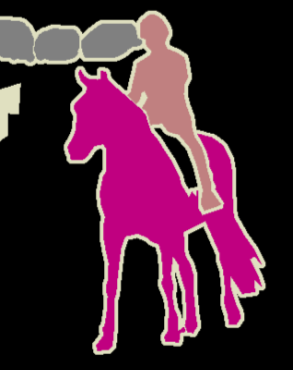
\includegraphics[width=\textwidth]{plots/segmentationTruth.png}
		\caption{Segmentation}
        \end{subfigure}
	\caption[Segmentation of an image]{Segmentation of an image with five classes. Image courtesy of~\cite{Long2015}}
	\label{fig:imageSegmentation}
\end{figure}

Convolutional networks are specially apt for image segmentation: we can transform each fully connected layer into a convolutional layer by padding the input volume to preserve spatial dimensions~\footnote{Padding by $\lfloor (f_s-1)/2\rfloor$ where $f_s$ is the filter size.} creating a network that is able to segment images of any size, albeit, due to subsampling in the pooling layers, it produces a coarse segmentation that needs to be upsampled to match the size of the original image.
%Adding zero-padding to each fully connected layer~\footnote{As with convolutional layers, padding the input volume by $\lfloor (f_s-1)/2\rfloor$ where $f_s$ is the filter size.} creates a convolutional network that is able to segment images of any size, albeit, due to subsampling in the pooling layers, produces a coarse segmentation that needs to be upsampled to match the size of the original image.
%Convolutional networks automatically behave this way when presented with a bigger image than those used for training, albeit, due to subsampling in the pooling layers, they produce a coarse segmentation that needs to be upsampled to match the size of the original image.
For instance, a convolutional network trained with $32\times 32$ images and two pooling layers (that reduce the input by a factor of 4) acts as a $32 \times 32$ filter with stride 4 so for a $256 \times 256$ image it will produce a $64 \times 64$ segmentation that needs to be upsampled by a factor of 4 to recover the original dimensions.
\begin{comment}
We could also set a stride of 4 in the first (converted) fully connected layer to get score matrices of size $3\times 3$ for each 9 non-overlapping $32\times 32$ partitions of the original image. It works exactly as if we applied the convolutional network to the original image at a stride of 32 but does all computations in just one pass.
if we augment the stride of the firs fully connected layer we can compute coarser segmentations or
\end{comment}
%For training, the loss function sums the loss over all pixels; to account for the mismatch between the output of the network and the ground truth image (labels), which has the dimensions of the original image, we downsample the ground truth image or append an upsampling layer at the end of the network. This layer computes a differentiable function either fixed such as bilinear interpolation or learned such as a linear mapping; adding this upsampling layer forms a \emph{fully convolutional network}~\cite{Long2015}.
To account for the difference in size between the output of the network and the label image---the ground truth segmentation\textemdash, we downsample the label image or append an upsampling layer at the end of the network~\cite{Long2015}; the additional layer computes a differentiable function either fixed such as bilinear interpolation or learned such as a linear mapping.
%; this forms a \emph{fully convolutional network}~\cite{Long2015}.
%Setting the loss function to sum the loss over all pixels completes the modifications needed.
%Subsampling, however, afects the granularity of the predicted segmentation.
Alternatively, we could remove pooling layers and use \emph{dilated convolutions}, filters with spaces between any two values (Fig.~\ref{fig:DilatedConvolutions}), thus enlarging the receptive field of the filter as pooling would do but keeping the spatial dimensions of the volume and the number of parameters fixed~\cite{Yu2016}.
\begin{figure}[h]
	\centering
	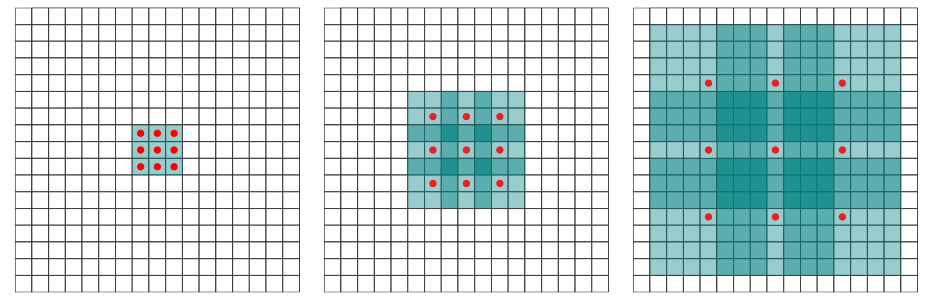
\includegraphics[width=0.8\textwidth]{plots/dilatedConv.png}
	\caption[Example of dilated convolutions]{Example of a $3\times3$ convolutional filter at different dilations: zero, one and three. The spatial dimensions of the input volume are represented as a black grid, red dots signal the places where the filter is applied and the green shadows represent the effective receptive field of the filter. Courtesy of~\cite{Yu2016}.}
	\label{fig:DilatedConvolutions}
\end{figure}

Lastly, the loss function sums the loss over all pixels so the network performs a single gradient update after one example segmentation. Convolutional networks transform image segmentation into an end-to-end, learnable task.

% Results are evaluated [using|with] the metrics [defined |introduced|used] [for|in] [classification|section] [computed|applied] pixelwise..
% [To evaluate results|For evaluation,|] we [compute|use|measure] [the average of|image-wise|] [classification|evaluation] metrics [for each|per|in each] [image|segmentation] and average [over all [of them| segmentations| images]]; for instance, [pixel] accuracy [measures|is] the (average) proportion of correctly classified pixels in [one|an] [image.
%To evaluate results, we use classification metrics (Sec.~\ref{sec:Classification}) averaged over all images; for instance, pixel accuracy is the average proportion of correctly classified pixels per image. Other metrics are calculated similarly.
%To evaluate results, we measure a classification metric per segmentation and average its result over all segmentations; for instance, pixel accuracy measures the (expected) proportion of correctly classified pixels in a segmentation.
%We use \emph{pixel accuracy}, the proportion of correctly classified pixels in a segmentation, to evaluate results. Evaluation metrics, including pixel accuracy, are the average value of a classification metric (Sec.~\ref{sec:Classification}) measured on segmentations produced for the test set. 
%To evaluate results, we compute the average value of a classification metric (Sec.~\ref{sec:Classification}) measured on segmentations produced for the test (or validation) set. \emph{Pixel accuracy}, for instance, estimates the (expected) proportion of correctly classified pixels in a segmentation.
%Evaluation metrics are the average value of a classification metric (Sec.~\ref{sec:Classification}) measured on segmentations produced for the test (or validation) set. \emph{Pixel accuracy}, for instance, estimates the (expected) proportion of correctly classified pixels in a segmentation.
%To evaluate the model, we measure a classification metric (Sec.~\ref{sec:Classification}) on segmentations of images in the test set and average the results;
To evaluate the model, we evaluate each segmentation using standard metrics (Sec.~\ref{sec:Classification}) and average over all test images. \emph{Pixel accuracy}, for instance, is the average proportion of correctly classified pixels in an image.
%[Other metrics are calculated| We calculate other metrics] [similarly|in a similar fashion]. 
Another popular metric, \emph{intersection over union} or \emph{IOU}, is calculated for a single segmentation as $TP/(TP+FP+FN)$ (Tab.~\ref{tab:ConfusionMatrix}).
%IOU = DC/(2-DC) (DC: Dice coefficient)
%DC = 2IOU/(IOU+1)
In medical diagnosis, the \emph{free-response operating curve} or {FROC curve} evaluates the performance of a radiologist or CAD system at localizing lesions. For varying thresholds, the FROC curve plots the sensitivity of the system (proportion of lesions correctly localized) versus the number of false positives commited per image. We can compare between models using their sensitivity at a fixed number of false positives per image, for instance, sensitivity at 1 FP/image.

If we are interested in a particular class, e.g. object vs. background, we present a single score map showing its probability distribution across every position in the image. We can refine this map using gaussian smoothing, cluster-based thresholding and conditional random fields among other techniques. Finally, to produce a segmentation we threshold the post-processed map at some specific value, which can be chosen using a validation set.
